\documentclass[10pt,twocolumn,letterpaper]{article}

% CVPR-inspired two-column report layout. This source is self-contained
% and uses standard LaTeX packages rather than requiring cvpr.sty.
\usepackage[margin=0.72in, columnsep=0.24in]{geometry}
\usepackage{times}
\usepackage{graphicx}
\usepackage{amsmath}
\usepackage{booktabs}
\usepackage{url}
\usepackage[hidelinks]{hyperref}
\usepackage{caption}
\usepackage{enumitem}
\setlength{\parindent}{1em}
\setlength{\parskip}{0.15em}
\captionsetup{font=small}
\setlist{nosep,leftmargin=*}
\pagestyle{plain}

\title{\bf Raw-Pixel Face Recognition with Decision Trees, Bagging, SAMME Boosting, and Bootstrap Analysis}

\author{
Harshid Bhupendra Rawal\\
Roll Number: m26ecm504\\
\texttt{https://github.com/harshitrawal513/Ml-Assignment-final}\\
Experiment code snapshot: \texttt{38ec520}
}

\begin{document}
\maketitle

\begin{abstract}
This report evaluates tree-based ensemble methods for multiclass face recognition using the Olivetti Faces dataset and raw flattened pixel features. A fixed identity-stratified split assigns six images per identity to training, two to validation, and two to testing, with random seed 26504. A decision-tree baseline is compared with a from-scratch bootstrap aggregation (bagging) implementation, including out-of-bag (OOB) evaluation and robustness to a centered image mask. A multiclass SAMME AdaBoost implementation is tuned using validation accuracy across tree depths and boosting rounds. Finally, 30 within-identity bootstrap training sets are used to examine individual-model accuracy, ensemble majority voting, and a multiclass prediction-variance measure. Bagging achieves 87.50\% clean test accuracy compared with 61.25\% for the baseline. The best SAMME validation configuration uses depth four and 100 rounds, reaching 45.00\% clean test accuracy. Masking the central rows and columns substantially degrades all methods, showing that these models rely strongly on information removed by the mask.
\end{abstract}

\section{Introduction}
Face recognition is a challenging multiclass classification task because images of the same identity vary in expression, lighting, and details. This study compares a single decision tree with two ensemble strategies: bootstrap aggregation and multiclass adaptive boosting. It also examines how decision-tree complexity and bootstrap resampling affect predictive performance.

The experiments intentionally use raw pixel values without dimensionality reduction. Each $64\times64$ grayscale image is flattened to a 4096-dimensional feature vector. All methods use the same saved training, validation, and test indices to keep comparisons consistent.

\section{Dataset and Experimental Protocol}
\subsection{Dataset}
The Olivetti Faces dataset contains 400 grayscale images from 40 identities, with 10 images per identity. Each image is $64\times64$ pixels. Pixel features are flattened directly into vectors of length 4096; no PCA or other feature transformation is applied.

\subsection{Fixed split and seed}
The random seed is 26504, obtained from the numeric characters of the roll number \texttt{m26ecm504}. Using NumPy's \texttt{default\_rng}, images are shuffled independently within each identity. Six images per identity are assigned to training, two to validation, and two to test, yielding 240 training, 80 validation, and 80 test images. The split is saved to \texttt{data/split\_indices.npz} and reused by all experiments.

\subsection{Masked test set}
Robustness is evaluated by masking the central image region: rows 24--39 and columns 24--39 are set to zero. Models are trained on clean training images only; the mask is applied to test images at evaluation time. Thus, the masked results measure test-time corruption rather than training with masked examples.

\section{Methods}
\subsection{Decision-tree baseline}
A single decision tree is trained on the 240 training examples and evaluated on validation, clean test, and masked test data. This provides a baseline for the ensemble experiments.

\subsection{Bootstrap aggregation}
Bagging trains 100 decision trees. Each tree is fitted to a bootstrap sample drawn with replacement from the training set. For each training example, predictions from trees that did not include that example are accumulated to compute out-of-bag accuracy. The implementation also reports OOB coverage, pairwise disagreement among tree predictions on the test set, and the mean vote margin. The vote margin is the difference between the largest and second-largest class vote fractions.

\subsection{Multiclass SAMME AdaBoost}
SAMME is implemented from scratch using decision trees as weak learners. At each boosting round, a tree is fitted using the current sample weights. Its weighted error determines its contribution to the ensemble, and sample weights are updated to emphasize misclassified examples. Tree depths in $\{1,2,3,4\}$ and round counts in $\{10,25,50,100\}$ are evaluated. The configuration with the highest validation accuracy is selected; the test set is used only for final evaluation.

\subsection{Within-identity bootstrap analysis}
For each depth in $\{1,2,3,4,\text{unlimited}\}$, 30 bootstrap training sets are generated. Each identity's six training examples are resampled with replacement separately, retaining six sampled examples per identity. For every depth, we report the mean and standard deviation of individual-model test accuracy, majority-vote accuracy, and multiclass prediction variance. For test example $i$, let $p_{ic}$ be the fraction of bootstrap models predicting class $c$. The variance measure is
\[
V = \frac{1}{N}\sum_{i=1}^{N}\left(1-\sum_c p_{ic}^{\,2}\right).
\]
This measures disagreement in the empirical class-prediction distribution across bootstrap models. The aggregate error $1-\text{accuracy}_{\text{majority vote}}$ is reported as an error proxy, not as a formal statistical estimate of bias.

\section{Results}
\subsection{Baseline and bagging}
Table~\ref{tab:q1} summarizes the baseline and bagging performance. Bagging improves clean test accuracy by 26.25 percentage points relative to the single-tree baseline. The OOB estimate is computed only from trees for which each training example was out of bag.

\begin{table}[t]
\centering
\caption{Decision-tree baseline and bagging results.}
\label{tab:q1}
\begin{tabular}{lrr}
\toprule
Metric & Baseline & Bagging\\
\midrule
Validation accuracy & 57.50\% & 86.25\%\\
Clean test accuracy & 61.25\% & 87.50\%\\
Masked test accuracy & 2.50\% & 6.25\%\\
\bottomrule
\end{tabular}
\end{table}

The bagging implementation reports OOB accuracy of 77.08\% with 100\% OOB coverage. Mean pairwise disagreement on test predictions is 0.7723, while the mean vote margin is 0.2895. The high disagreement indicates that individual trees often differ; aggregation can still improve accuracy by combining their predictions.

\begin{figure}[t]
\centering
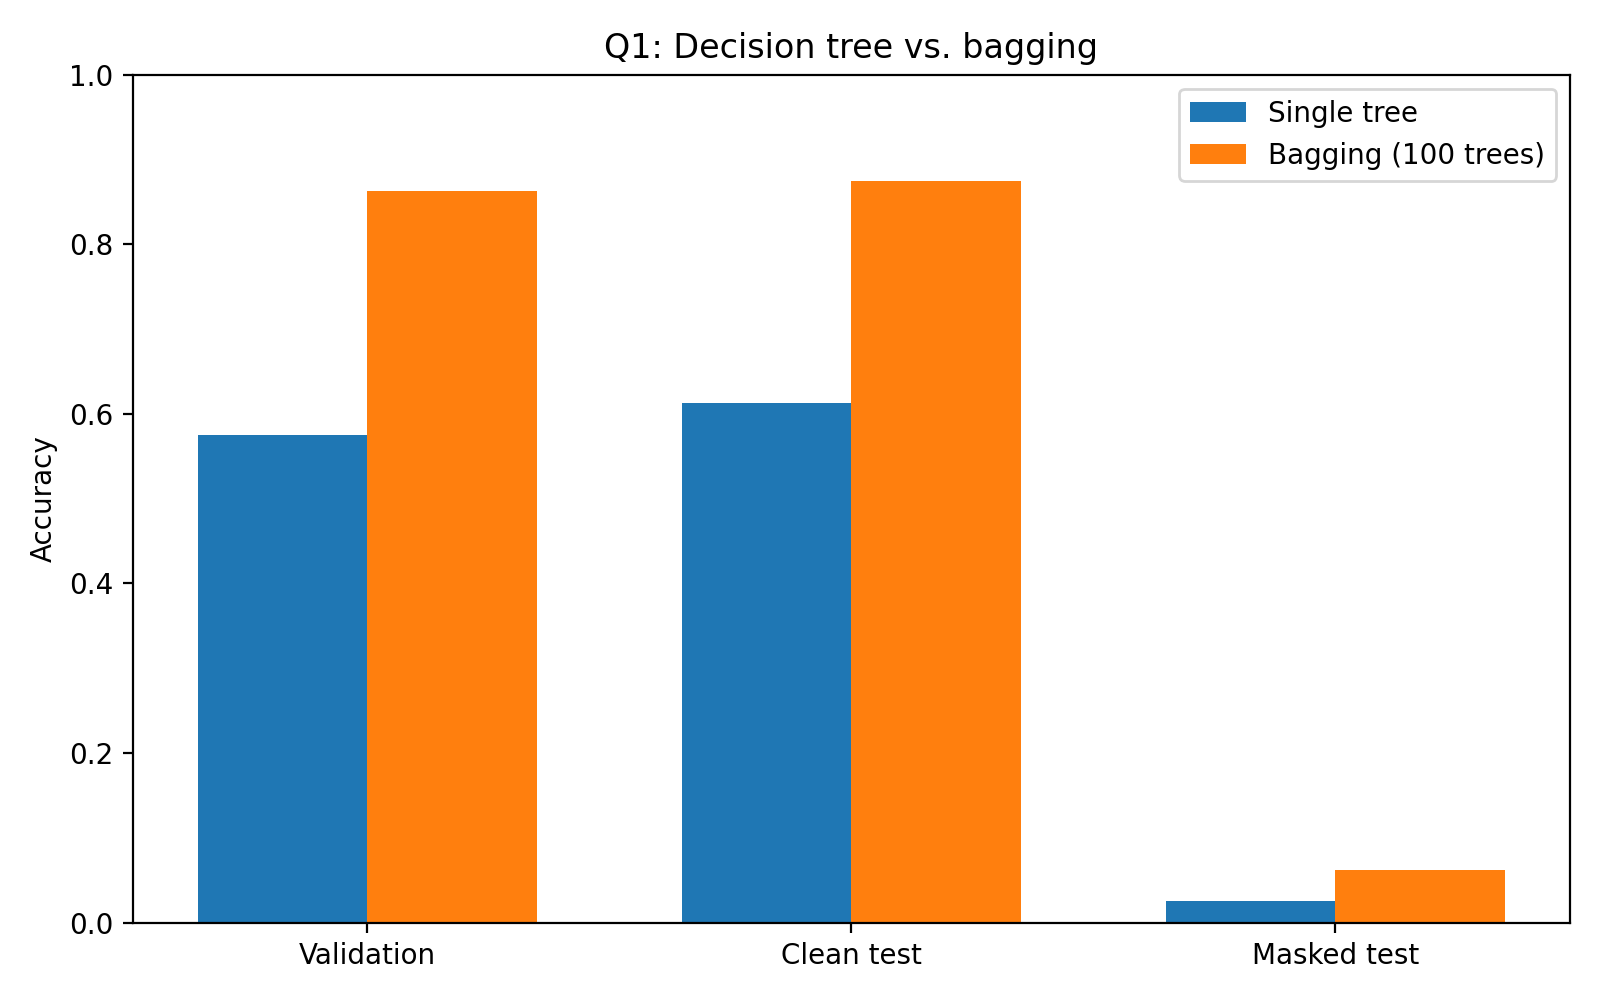
\includegraphics[width=\linewidth]{../figures/q1_accuracy.png}
\caption{Validation and test accuracy for the decision-tree baseline and bagging.}
\label{fig:q1}
\end{figure}

\subsection{SAMME validation tuning}
Table~\ref{tab:q2} gives validation accuracy for all tested configurations. The best validation score is 36.25\%, obtained with depth four and 100 rounds. This configuration reaches 45.00\% clean test accuracy and 2.50\% masked test accuracy.

\begin{table}[t]
\centering
\caption{SAMME validation accuracy by tree depth and boosting rounds.}
\label{tab:q2}
\begin{tabular}{lrrrr}
\toprule
Depth & 10 & 25 & 50 & 100\\
\midrule
1 & 2.50 & 5.00 & 8.75 & 15.00\\
2 & 7.50 & 15.00 & 8.75 & 17.50\\
3 & 10.00 & 18.75 & 22.50 & 31.25\\
4 & 20.00 & 22.50 & 31.25 & 36.25\\
\bottomrule
\end{tabular}
\end{table}
\noindent{\footnotesize Values are percentages.}

Validation performance generally improves with depth and more rounds, although the depth-two score at 50 rounds is lower than at 25 rounds. The tuned SAMME model remains less accurate than bagging on this dataset and split.

\begin{figure}[t]
\centering
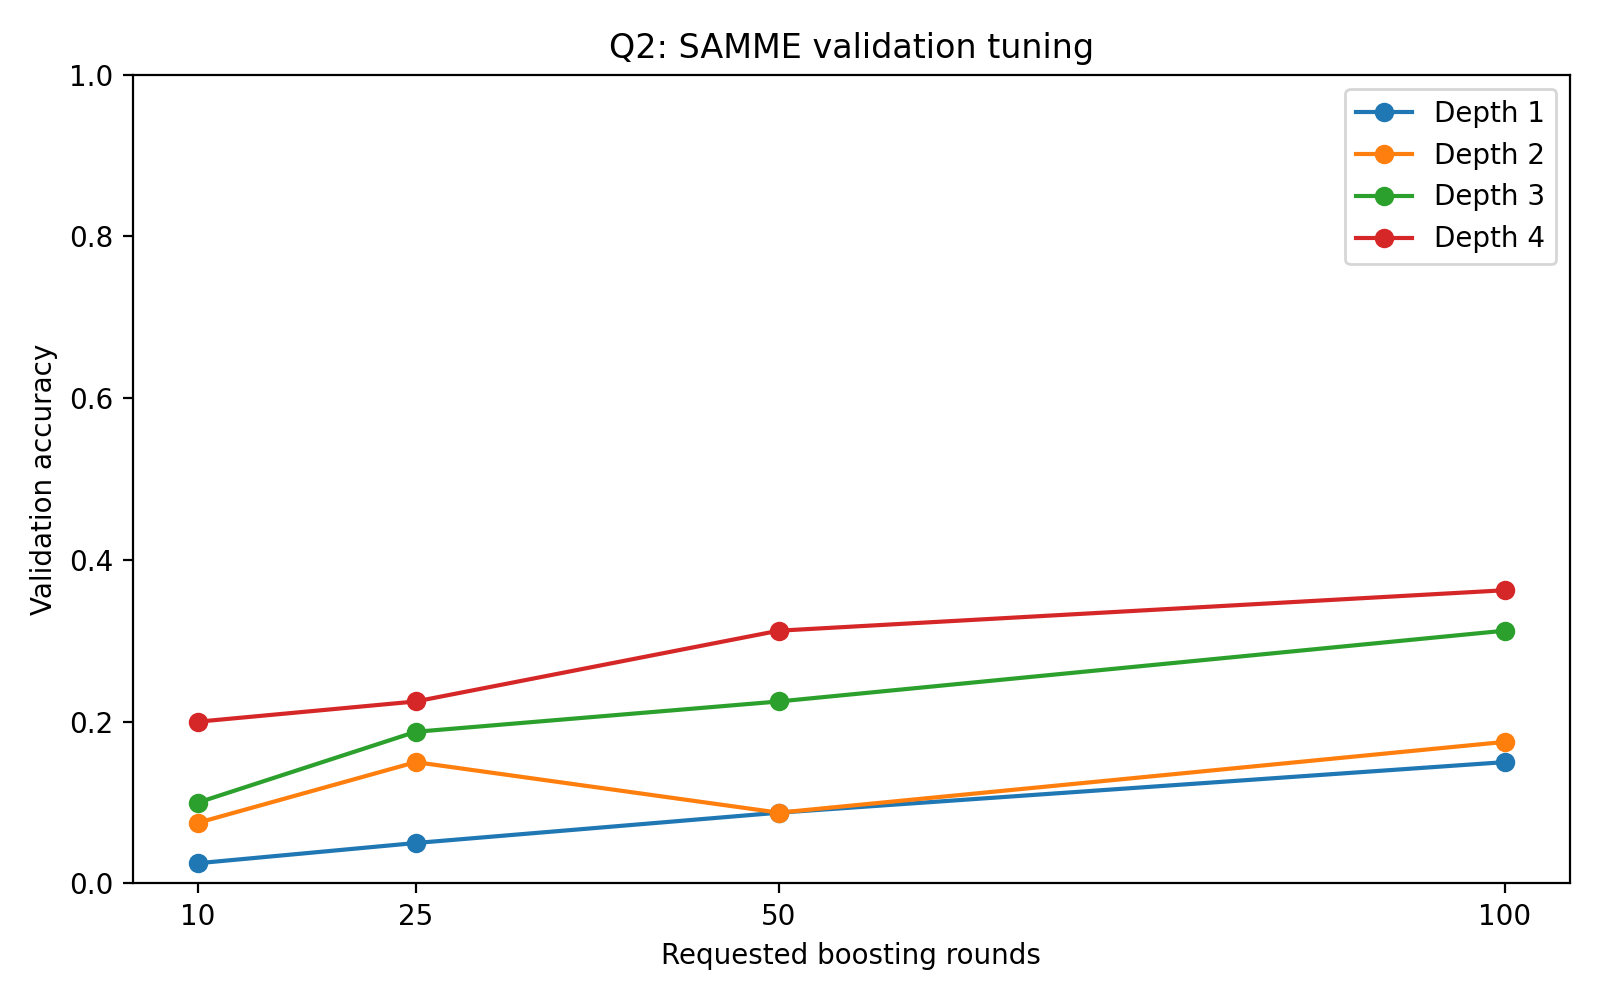
\includegraphics[width=\linewidth]{../figures/q2_tuning.png}
\caption{SAMME validation accuracy across depths and boosting rounds.}
\label{fig:q2}
\end{figure}

\subsection{Bootstrap accuracy and variance}
Table~\ref{tab:q3} summarizes the 30 within-identity bootstrap models for each depth. Unlimited-depth trees have the highest mean individual accuracy (48.50\%) and majority-vote accuracy (78.75\%). Shallow trees perform poorly on this 40-class task. The standard deviation in individual accuracy is also largest for unlimited-depth trees among the tested settings.

\begin{table}[t]
\centering
\caption{Within-identity bootstrap analysis over 30 resamples.}
\label{tab:q3}
\begin{tabular}{lrrrr}
\toprule
Depth & Mean acc. & Std. & Vote acc. & Variance\\
\midrule
1 & 4.50 & 0.76 & 2.50 & 0.1068\\
2 & 6.21 & 1.27 & 3.75 & 0.1423\\
3 & 8.75 & 1.41 & 5.00 & 0.1212\\
4 & 10.08 & 1.33 & 5.00 & 0.1521\\
Unlimited & 48.50 & 4.82 & 78.75 & 0.6210\\
\bottomrule
\end{tabular}
\end{table}
\noindent{\footnotesize Accuracy and standard deviation are percentages; variance is dimensionless.}

The high majority-vote accuracy for unlimited-depth trees indicates that aggregating predictions from resampled models can be substantially more effective than relying on a typical individual model. Its higher variance value also reflects greater diversity in predictions across bootstrap models. These observations should be interpreted cautiously because the test set contains only 80 examples.

\begin{figure}[t]
\centering
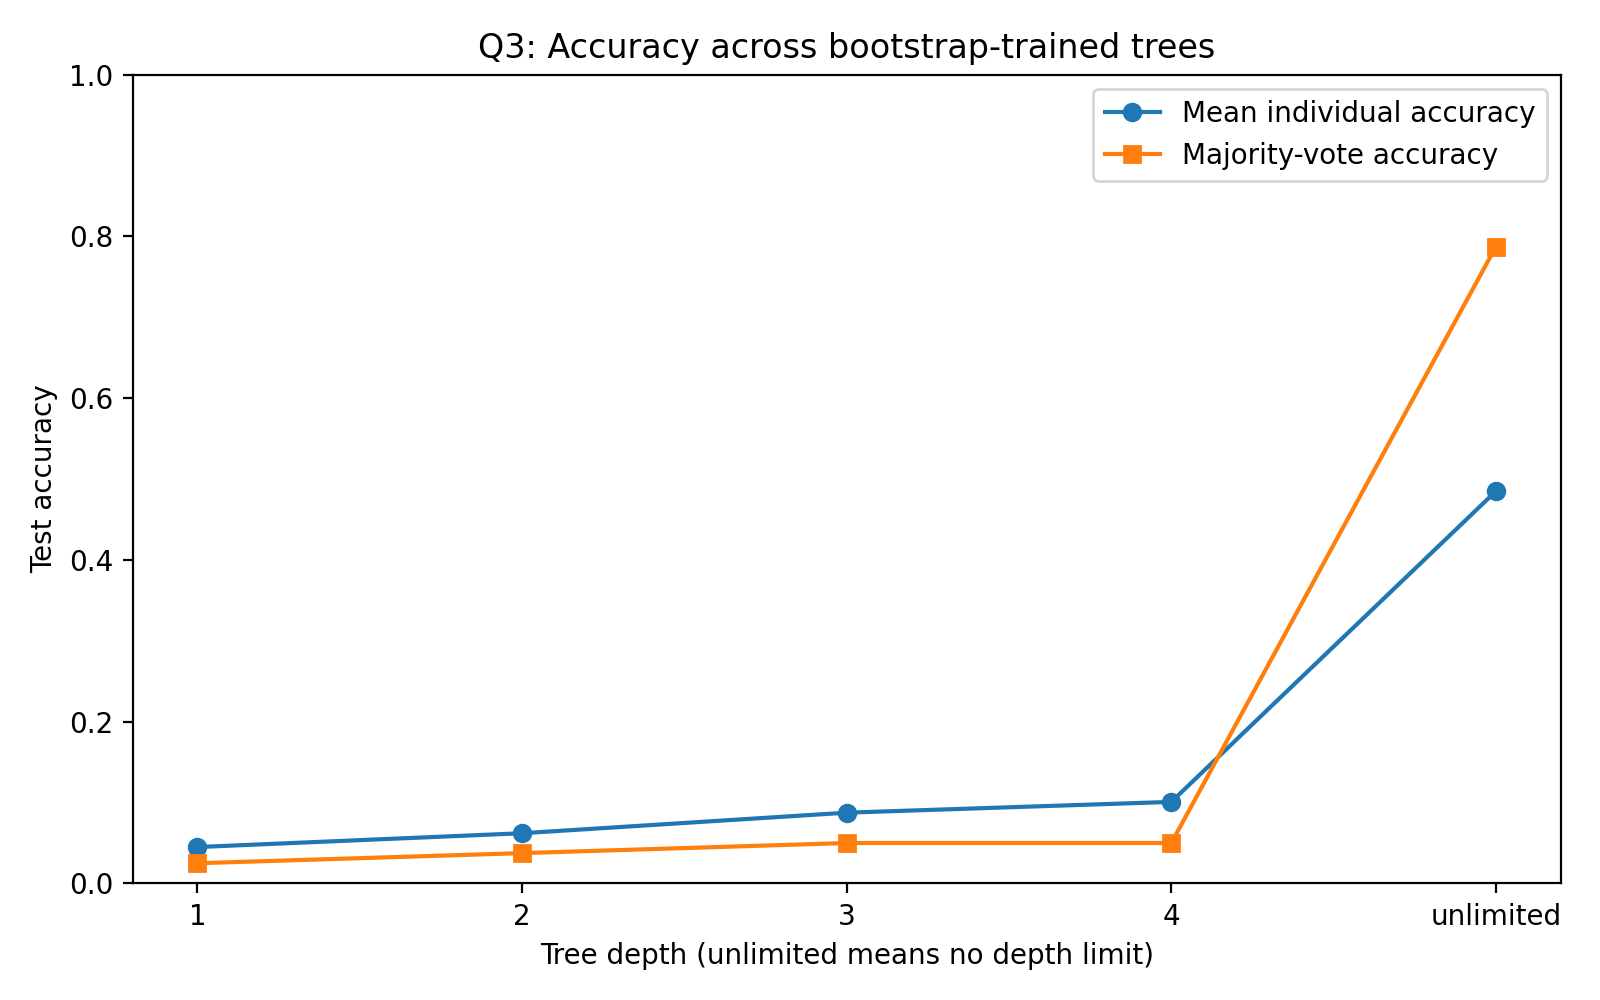
\includegraphics[width=\linewidth]{../figures/q3_accuracy.png}
\caption{Mean individual accuracy and majority-vote accuracy across tree depths.}
\label{fig:q3acc}
\end{figure}

\begin{figure}[t]
\centering
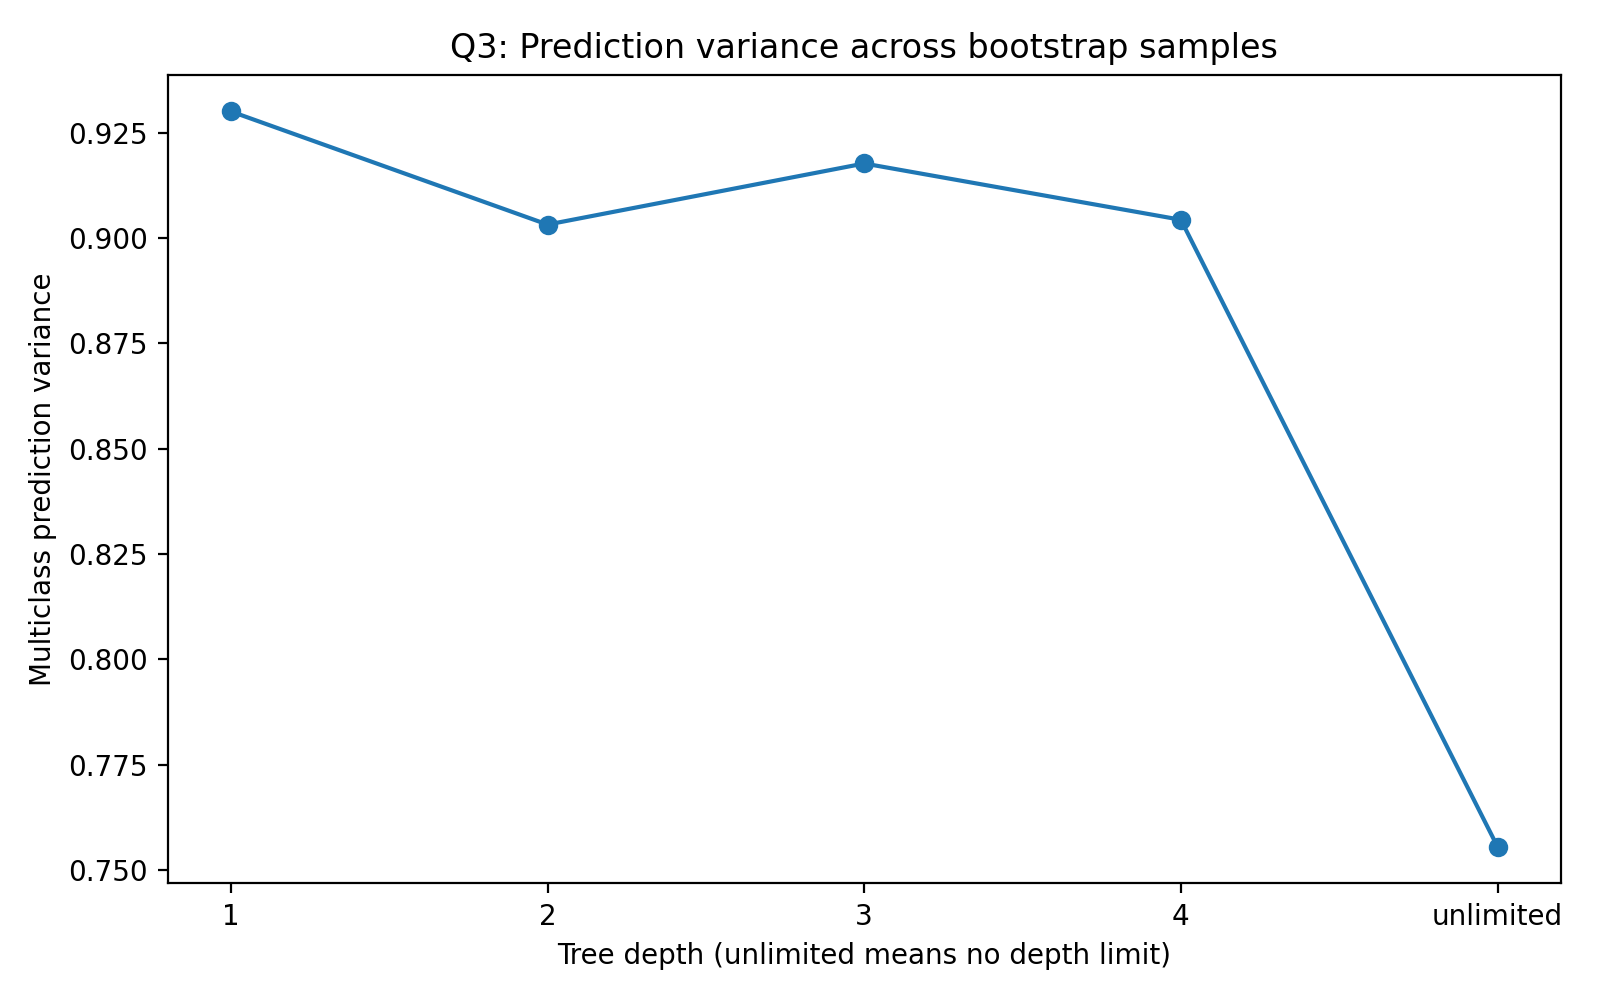
\includegraphics[width=\linewidth]{../figures/q3_variance.png}
\caption{Multiclass prediction variance across tree depths.}
\label{fig:q3var}
\end{figure}

\subsection{Robustness to masking}
The central mask causes a substantial accuracy drop for every evaluated method. The baseline falls from 61.25\% clean test accuracy to 2.50\% masked accuracy; bagging falls from 87.50\% to 6.25\%. The selected SAMME model reaches only 2.50\% on the masked test set. This suggests that the learned decision rules depend strongly on pixel information in the removed region. Since training uses only clean images, these results do not measure robustness achievable through corruption-aware training or augmentation.

\section{Discussion}
Three main observations emerge. First, bagging is the strongest of the evaluated standard methods on the clean test set, improving substantially over a single decision tree. Second, SAMME benefits from deeper weak learners and longer boosting runs in validation tuning, but does not match bagging in this experiment. Third, the within-identity bootstrap experiment shows a large difference between individual and majority-vote accuracy for unlimited-depth trees, illustrating the potential benefit of aggregation.

The masked-test results expose an important limitation: good clean accuracy does not imply robustness to structured occlusion. A follow-up study could compare clean-only training against augmentation or training with masked images, while keeping the test split fixed.

\section{Limitations}
The evaluation set contains only 80 images, with two test images per identity, so individual accuracy estimates are coarse and can vary noticeably. Only raw pixel features are used, without PCA, alignment, or learned representations. The bias--variance analysis uses an empirical multiclass prediction-dispersion measure and an aggregate-error proxy; neither should be interpreted as a formal decomposition of expected classification error into statistical bias and variance. Finally, the masked test corruption is a single deterministic central mask and does not represent all possible occlusions.

\section{Conclusion}
Under a fixed identity-stratified split and raw pixel features, bagging achieves the best clean test accuracy at 87.50\%, compared with 61.25\% for the decision-tree baseline and 45.00\% for the best validation-selected SAMME model. The within-identity bootstrap study finds that unlimited-depth trees achieve 48.50\% mean individual test accuracy and 78.75\% majority-vote accuracy. All methods are highly sensitive to the central test-time mask, motivating future work on occlusion robustness.

\begin{thebibliography}{9}
\bibitem{olivetti}
AT\&T Laboratories Cambridge.
\newblock The ORL Database of Faces.
\newblock \url{https://cam-orl.co.uk/facedatabase.html}.

\bibitem{breiman}
L. Breiman.
\newblock Bagging predictors.
\newblock \emph{Machine Learning}, 24:123--140, 1996.

\bibitem{freund}
Y. Freund and R. E. Schapire.
\newblock A decision-theoretic generalization of on-line learning and an application to boosting.
\newblock \emph{Journal of Computer and System Sciences}, 55(1):119--139, 1997.
\end{thebibliography}

\end{document}
